\documentclass[tikz,border=0.1cm,usenames,dvipsnames,convert={outext=.svg}]{standalone}
\usepackage{tikz,tikz-3dplot}
\usepackage{amsmath,amsthm}
\usepackage{amssymb}
\usepackage{amsfonts}
\usepackage{times}
\usepackage{svg}

\usetikzlibrary{positioning,arrows.meta,quotes}
\usetikzlibrary{shapes,snakes}
\usetikzlibrary{bayesnet}
\tikzset{>=latex}

\begin{document}
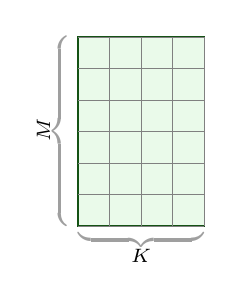
\begin{tikzpicture}
    % A
    \draw [thick,draw=LimeGreen!40!black] (.8*2,0*2) rectangle (1.6*2,1.2*2);
    \filldraw [fill=LimeGreen!10!white,draw=LimeGreen!40!black] (.8*2,0*2) rectangle (1.6*2,1.2*2);
    \draw [step=0.4, very thin, color=gray] (.8*2,0*2) grid (1.6*2,1.2*2);
    
    \draw (0.58*2,0.61*2) node[rotate = 90] {\scriptsize{\scriptsize$M$}};
    \draw (0.68*2,0.6*2) node[rotate = 270] {{\color{gray!75}$\underbrace{\hspace{2.4cm}}$}};

    \draw (0.6*4,-0.19*2) node[rotate = 0] {\scriptsize{\scriptsize$K$}};
    \draw (0.6*4,-0.09*2) node[rotate = 0] {{\color{gray!75}$\underbrace{\hspace{1.6cm}}$}};


    %\draw (-0.2,1,2) node[rotate = 270] {{\color{gray!75}$\underbrace{\hspace{2cm}}$}};
\end{tikzpicture}
\end{document}
